% \begin{itemize}
% \item component-based commissioning model
% \item control components to handle the commissioning of any existing
%   component in any language
% \item goals: programmable, composable, reusable, efficient
% \item composed of:
%   \begin{itemize}
%   \item meta-model
%   \item graphical language
%   \item concrete language
%   \item formal specification (next section)
%   \item formal operational semantics (next section)
%   \end{itemize}
% \item meta-models of assembly and components (add groups)
% \item example Apache/MariaDB with graphical and concrete syntax
% \item simplified explanation of the operational semantics (middleware)
% \item discussion on the goals
% \end{itemize}

%%%%%%%%%%%%%%%%%%%%%%%%%%
\subsection{Principles}

Madeus is a component-based commissioning model. More precisely Madeus
offers a way to model and coordinate the execution of complex
distributed software commissioning procedures. To this purpose, a
Madeus component is a type containing a set of places that represent
milestones of the commissioning, and a set of transitions that connect
the places together and represent actions to be performed between
milestones (\eg \texttt{apt-get install}, \texttt{docker pull}
etc.). If multiple transitions leave a place, a parallel execution is
automatically handled and synchronized by Madeus. A component may have
dependencies to other external components. Such dependencies are
declared through a well known object of component-based software
engineering: ports. Four types of ports, working in pairs, are
available in Madeus: service-provide and service-use, data-provide and
data-use ports. By using ports, each component type can be defined
independently and component instances can be connected later by
another developer, thus improving the separation of concerns and the
code reuse. Madeus components are called \emph{control} component as
they only intend to model the commissioning procedure of an already
existing piece of code (component, module or service etc.) of a
distributed software system.

The overall commissioning procedure of a distributed software system
is built by composition in an \emph{assembly} file, where component
types are instanciated and connected. Each component is handled
individually, thus introducing more parallelism (in addition to
parallel transitions). Two components connected by their respective
compatible ports will be automatically synchronized such that a
component cannot use a service or a data if the associated provide
port is not enabled.

\emph{As a result, Madeus offers the expressivity to get composable,
reusable and efficient commissioning procedures for complex
distributed software systems.}

\begin{figure}[tbp]
  \begin{center}
    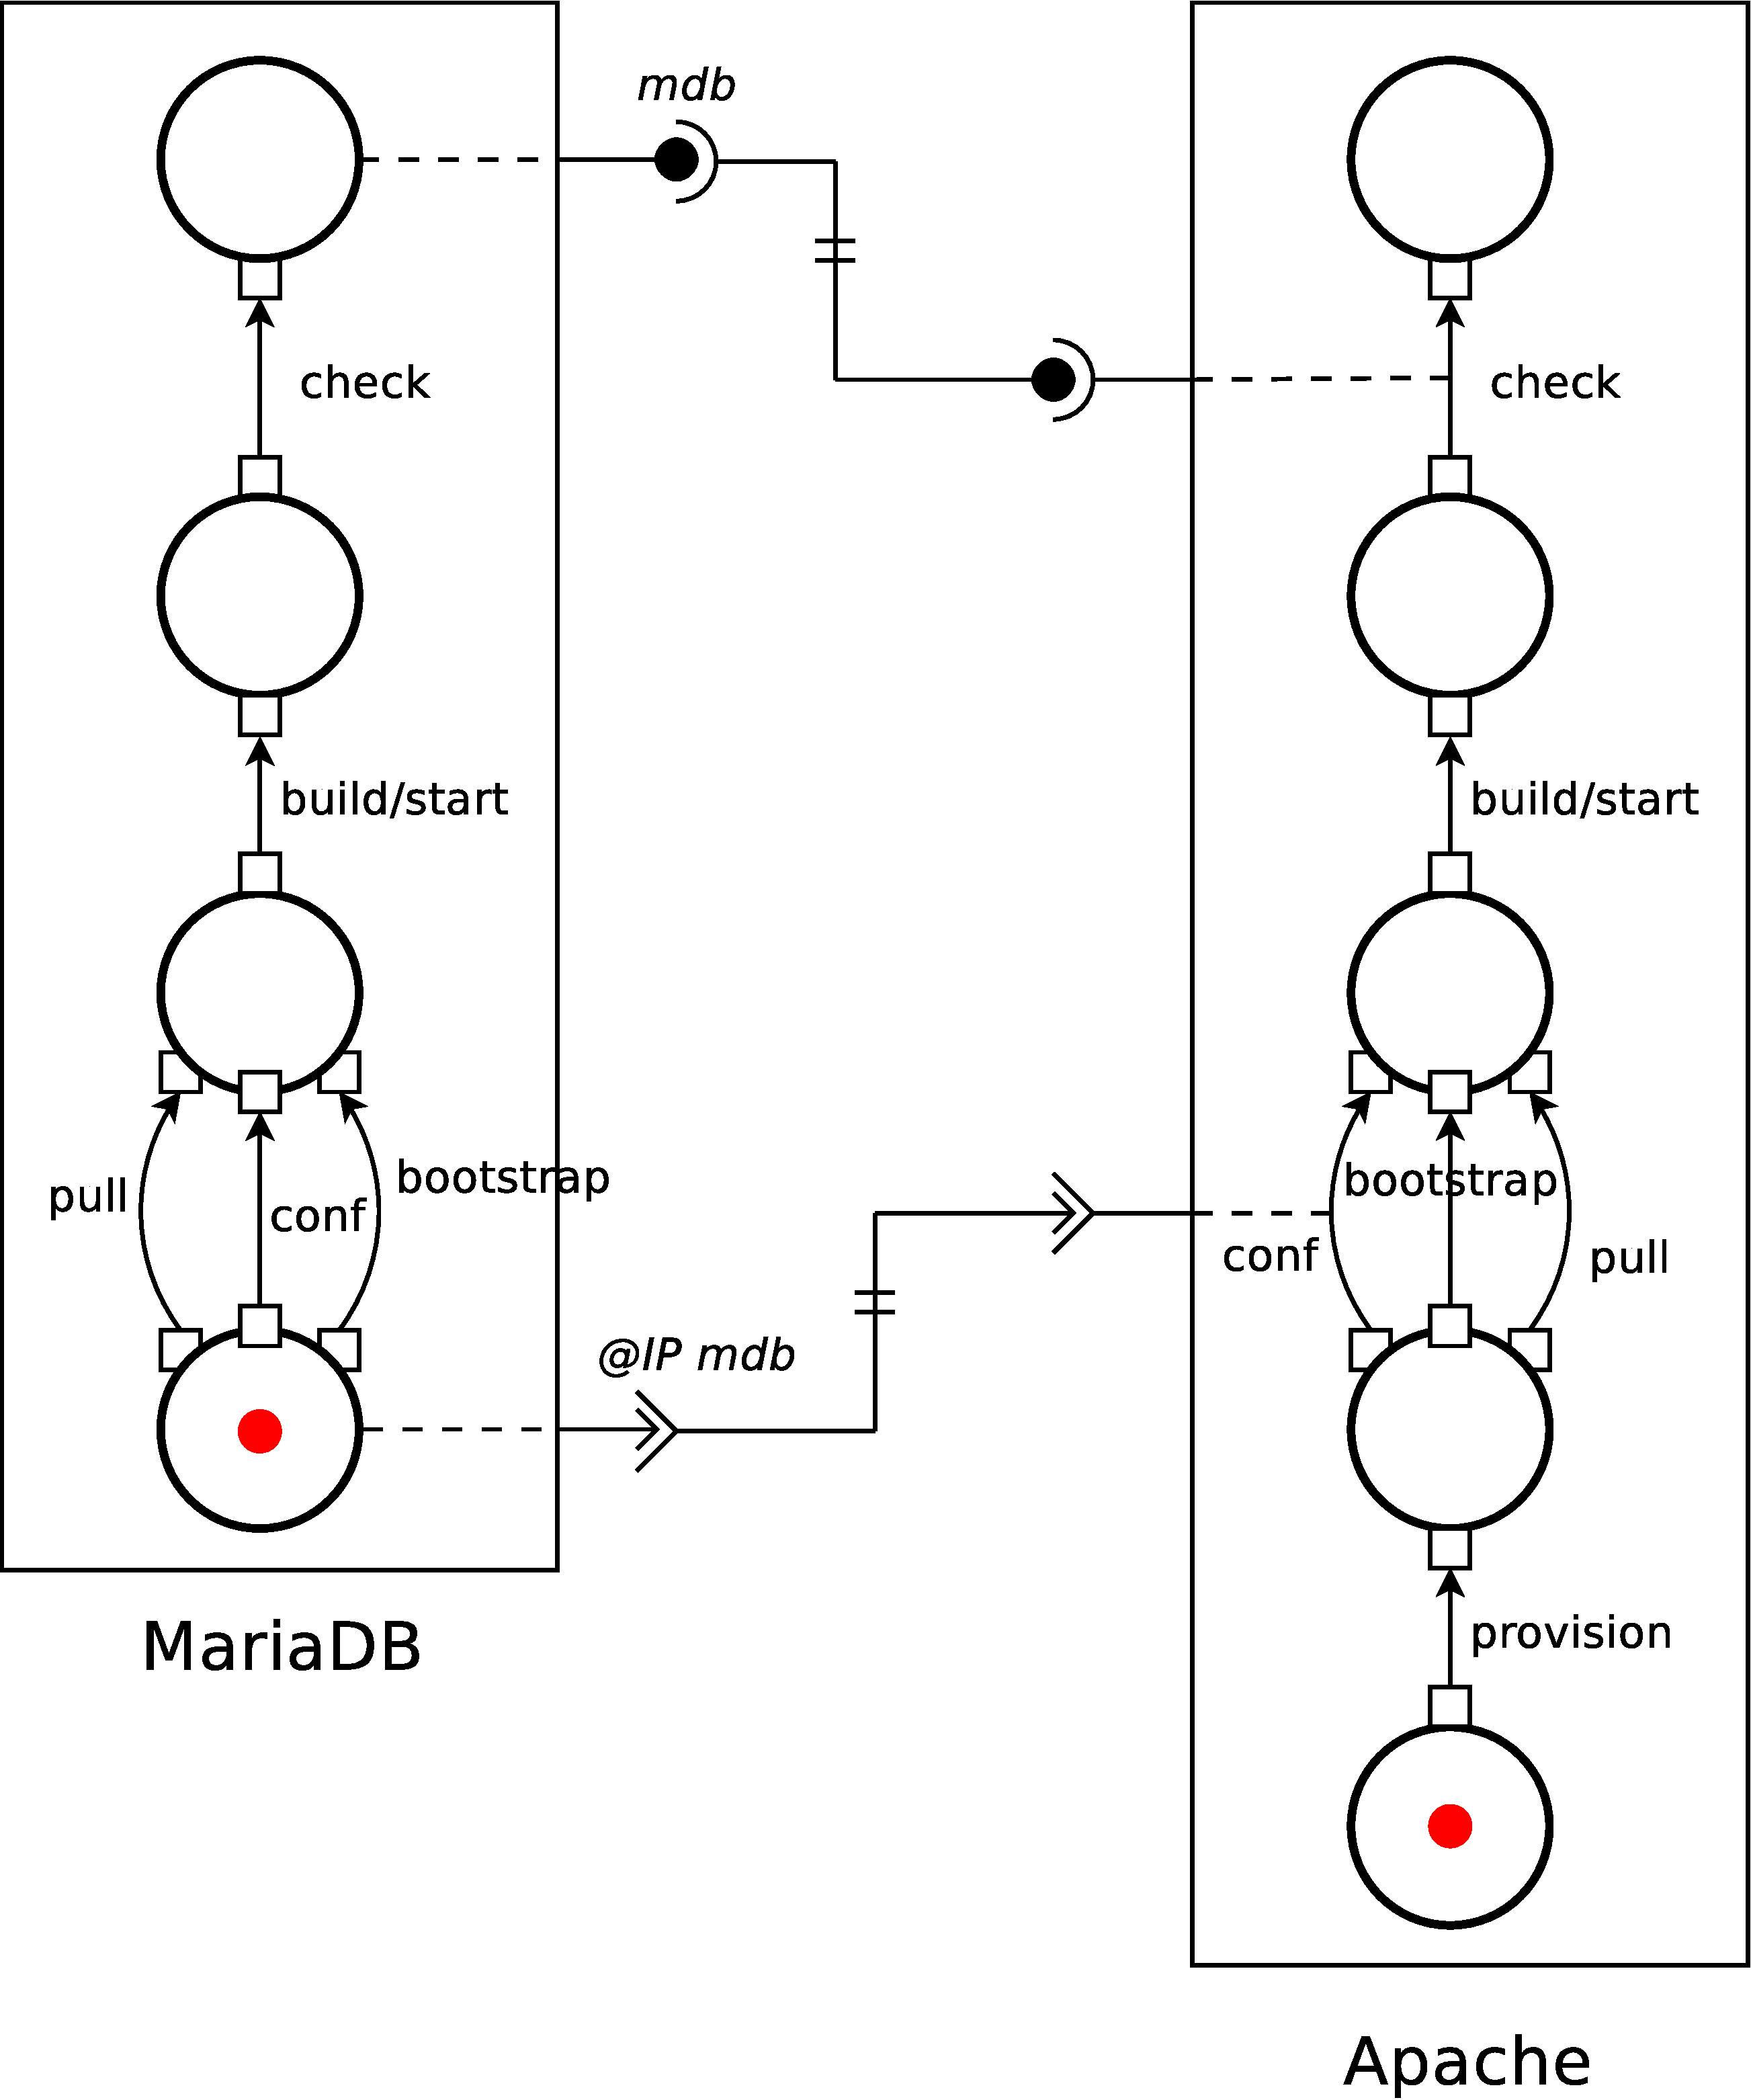
\includegraphics[width=0.35\linewidth]{./images/apachebdd.pdf}
  \end{center}
  \caption{Example of a commissioning assembly with two components
    Apache and MariaDB. Places are represented by circles, transitions
    by arrows between places, ports by either small black circles,
    semi-circles, outgoing or incoming arrows from components. Two
    initial red tokens are placed in each initial place of
    components.}
  \label{fig:example}
\end{figure}

\paragraph{Example}{ Figure~\ref{fig:example} depicts the Madeus
  commissioning of an Apache web server and a MariaDB database. This
  example is based on a real container-based deployment described by
  RedHat\footnote{\url{https://access.redhat.com/documentation/en-us/red_hat_enterprise_linux_atomic_host/7/html/getting_started_with_containers/install_and_deploy_an_apache_web_server_container}}%
  $^,$%
  \footnote{\url{https://access.redhat.com/documentation/en-us/red_hat_enterprise_linux_atomic_host/7/html/getting_started_with_containers/install_and_deploy_a_mariadb_container}}. Two
  component types are declared by using Madeus is this example: Apache
  and MariaDB. Apache contains four places, or millestones, while
  MariaDB contains five places. Some parallel transitions are declared
  for each of the component and can be observed in the figure. Both
  components have two ports. MariaDB provides both a data and a
  service (once installed), while Apache uses a service and a
  data. Figure~\ref{fig:example} shows the assembly of one Apache and
  one MariaDB instanciated from their component types. These instances
  are connected by their ports. Indeed, the Apache configuration need
  the IP adress of the MariaDB component, and the testing phase for
  Apache, called \texttt{check}, uses the MariaDB service.
}

In Madeus two kind of \emph{actors} are considered. First, the
developer of a control component, called \emph{dev-comp}, who may be
the same developer as the associated existing piece of code, or
another developer, or even a system operator or administrator. Second,
the developer of an assembly, called \emph{dev-ass}, who is typically
\HC[All]{le nom me fait rire :D} a system operator or administrator
who wants to write the overall commissioning procedure of a
distributed software system to deploy on its infrastructure. One
important difference bewteen Madeus and other approaches is its clear
separation of concerns between the commissioning of a single component
and the composition of an assembly, without taking care of the
commissioning of each component. Even if Ansible, Puppet and Chef, for
instance, offer properties close to composition (\eg roles, playbooks,
recipes etc.), the system operator still have to handle the correct
order of composition. The correct coordination, thus the correct order
of execution, is automatically guaranteed by Madeus by the composition
of the component instances. Such property has also been offered by
Aeolus~\cite{} but without parallelism within components.

%%%%%%%%%%%%%%%%%%%%%%%%%%
\subsection{Language}

\HC[Dim]{en cours}

Madeus is constituted of multiple elements. First, Madeus is a
language to model distributed software commissionings, thus Madeus is
a \emph{meta-model}. Madeus has been formalized~\cite{}, this
formalization will be detailed in Section~\ref{}. Second, Madeus is a
\emph{graphical language} that can be used to observe and understand
how a distributed software commissioning is modeled, but also to be
able to monitor the state of this procedure. Third, Madeus is equiped withq a
\emph{concrete language}, which is for now prototyped in
Python. Finally, Madeus is able to execute one assembly by following a
formal \emph{operational semantics}. In this sub-section we give an
overview of the meta-model, the concrete language and the execution
semantics of Madeus. Later Sections~\ref{} and~\ref{} will present the
formalization of Madeus.

% meta-model

% concrete language

% operational semantics
